
\documentclass[11pt]{article}
\usepackage[margin=1in]{geometry}
\usepackage{graphicx}
\usepackage{booktabs}
\usepackage{float}
\usepackage{hyperref}
\title{Monthly Gulf of Mexico OHC/TCHP Comparison\\Argo GDAC vs Same-Day RTOFS}
\date{}
\begin{document}
\maketitle

\section*{Overview}
This report documents a TEOS-10-backed collocation study carried out in the Gulf of Mexico
for 2024. For each month in January--March and August--October, we selected the top 5
Argo-coverage dates in the month, paired each Argo GDAC profile to the nearest same-day RTOFS
ocean column at the profile coordinates, and computed Tropical Cyclone Heat Potential (TCHP)
from both profiles using TEOS-10/GSW thermodynamics.

\section*{Method}
For each profile/column pair:
\begin{itemize}
\item Practical Salinity was converted to Absolute Salinity using \texttt{gsw\_SA\_from\_SP}.
\item Pressure/depth conversion used \texttt{gsw\_z\_from\_p} for Argo and \texttt{gsw\_p\_from\_z} for RTOFS.
\item Density used \texttt{gsw\_rho\_t\_exact} and heat capacity used \texttt{gsw\_cp\_t\_exact}.
\item The depth of the 26\,$^\circ$C isotherm ($D_{26}$) was found by linear interpolation.
\item TCHP was evaluated as $\int_0^{D_{26}} \rho(z) c_p(z) [T(z)-26]\,dz$ and reported in kJ/cm$^2$.
\end{itemize}

\section*{Monthly Summary}
\begin{table}[H]
\centering
\begin{tabular}{lrrrrrr}
\toprule
Month & Pairs & Floats & Dates & Argo mean & RTOFS mean & Mean diff \\
 &  &  &  & (kJ/cm$^2$) & (kJ/cm$^2$) & (Argo-RTOFS) \\
\midrule
Jan & 4 & 4 & 1 & 40.13 & 21.59 & 18.54 \\
Feb & 11 & 7 & 5 & 28.95 & 20.40 & 8.54 \\
Mar & 18 & 11 & 5 & 26.96 & 15.77 & 11.19 \\
Aug & 59 & 19 & 5 & 106.94 & 99.98 & 6.96 \\
Sep & 53 & 18 & 5 & 105.51 & 95.28 & 10.24 \\
Oct & 42 & 32 & 5 & 80.07 & 74.51 & 5.56 \\
\bottomrule
\end{tabular}
\end{table}

\section*{Seasonal Means}
\begin{table}[H]
\centering
\begin{tabular}{l r r r r}
\toprule
Window & Pairs & Argo mean & RTOFS mean & Mean diff \\
 &  & (kJ/cm$^2$) & (kJ/cm$^2$) & (kJ/cm$^2$) \\
\midrule
Jan-Mar & 33 & 29.22 & 18.02 & 11.20 \\
Aug-Oct & 154 & 99.12 & 91.42 & 7.70 \\
\bottomrule
\end{tabular}
\end{table}

\section*{Selected Sample Dates}
\begin{table}[H]
\centering
\begin{tabular}{l l r}
\toprule
Month & Date & Argo profiles \\
\midrule
Jan & 20240101 & 14 \\
Jan & 20240107 & 11 \\
Jan & 20240111 & 14 \\
Jan & 20240121 & 14 \\
Jan & 20240131 & 15 \\
Feb & 20240201 & 13 \\
Feb & 20240210 & 16 \\
Feb & 20240216 & 13 \\
Feb & 20240220 & 14 \\
Feb & 20240221 & 14 \\
Mar & 20240302 & 16 \\
Mar & 20240307 & 14 \\
Mar & 20240312 & 16 \\
Mar & 20240317 & 15 \\
Mar & 20240322 & 19 \\
Aug & 20240804 & 13 \\
Aug & 20240809 & 12 \\
Aug & 20240814 & 13 \\
Aug & 20240824 & 12 \\
Aug & 20240830 & 13 \\
Sep & 20240904 & 15 \\
Sep & 20240909 & 13 \\
Sep & 20240914 & 12 \\
Sep & 20240920 & 11 \\
Sep & 20240925 & 11 \\
Oct & 20241003 & 9 \\
Oct & 20241004 & 9 \\
Oct & 20241005 & 10 \\
Oct & 20241009 & 9 \\
Oct & 20241016 & 10 \\
\bottomrule
\end{tabular}
\end{table}

\section*{Figures}
\begin{figure}[H]
\centering
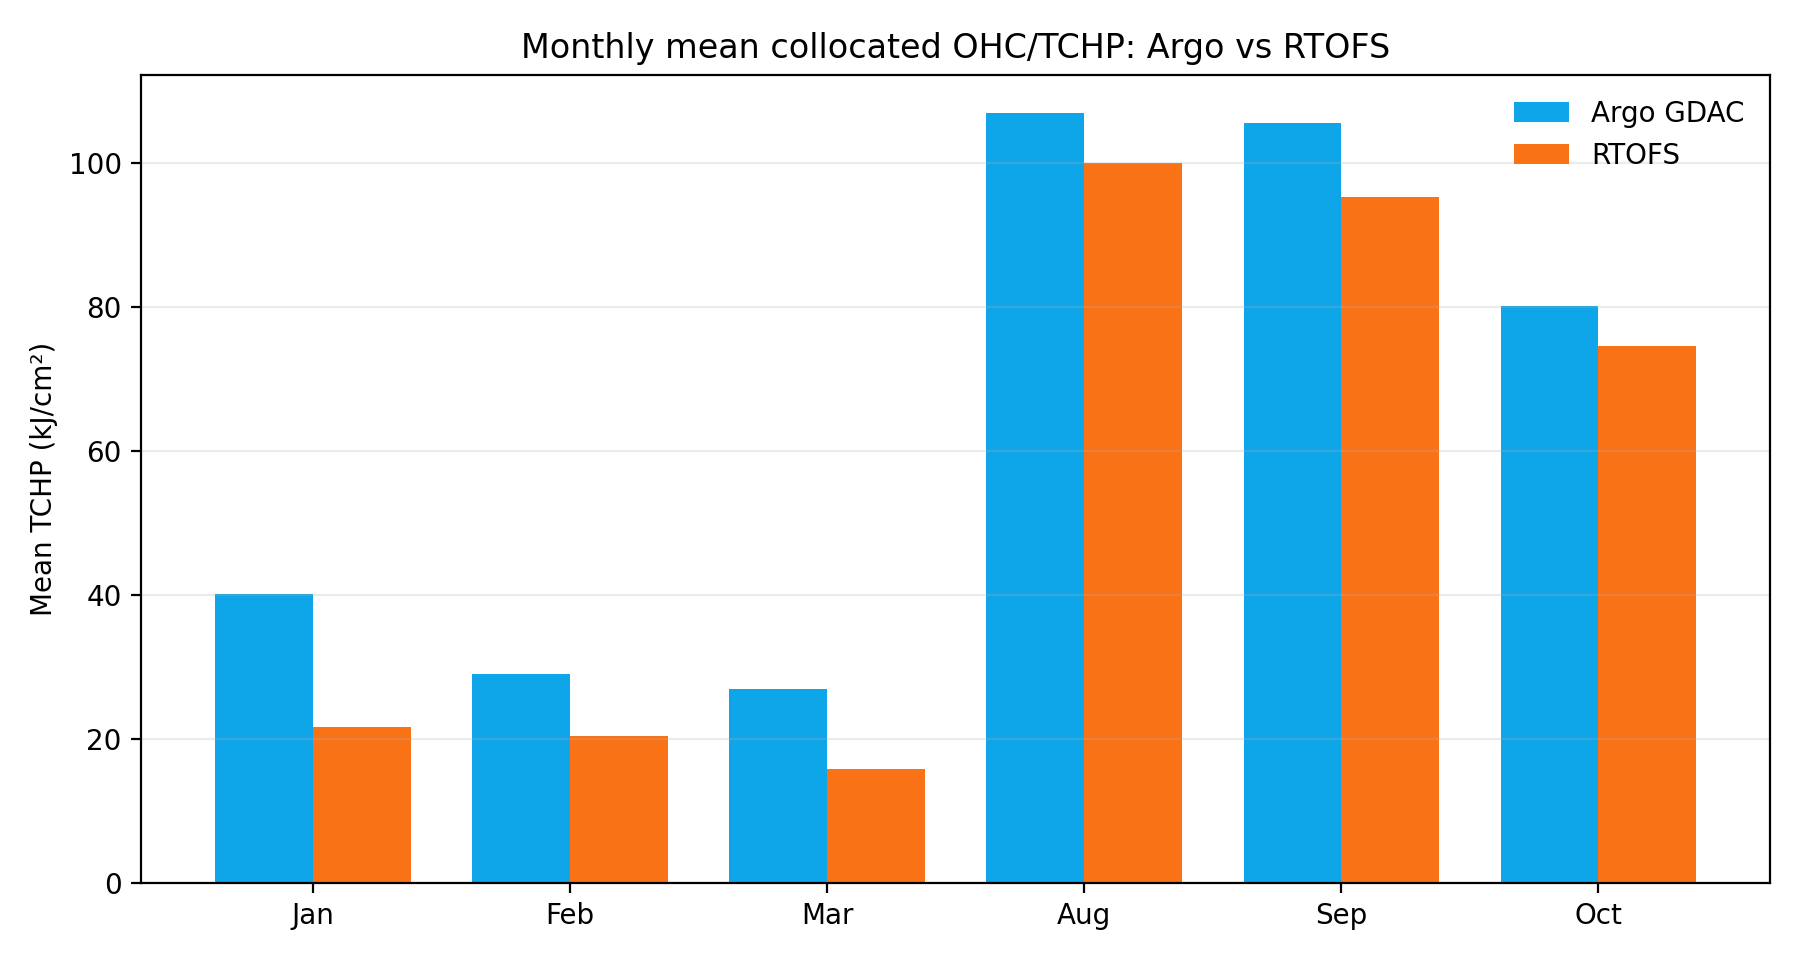
\includegraphics[width=0.92\textwidth]{monthly_means.png}
\caption{Monthly mean collocated TCHP for Argo GDAC and RTOFS.}
\end{figure}

\begin{figure}[H]
\centering
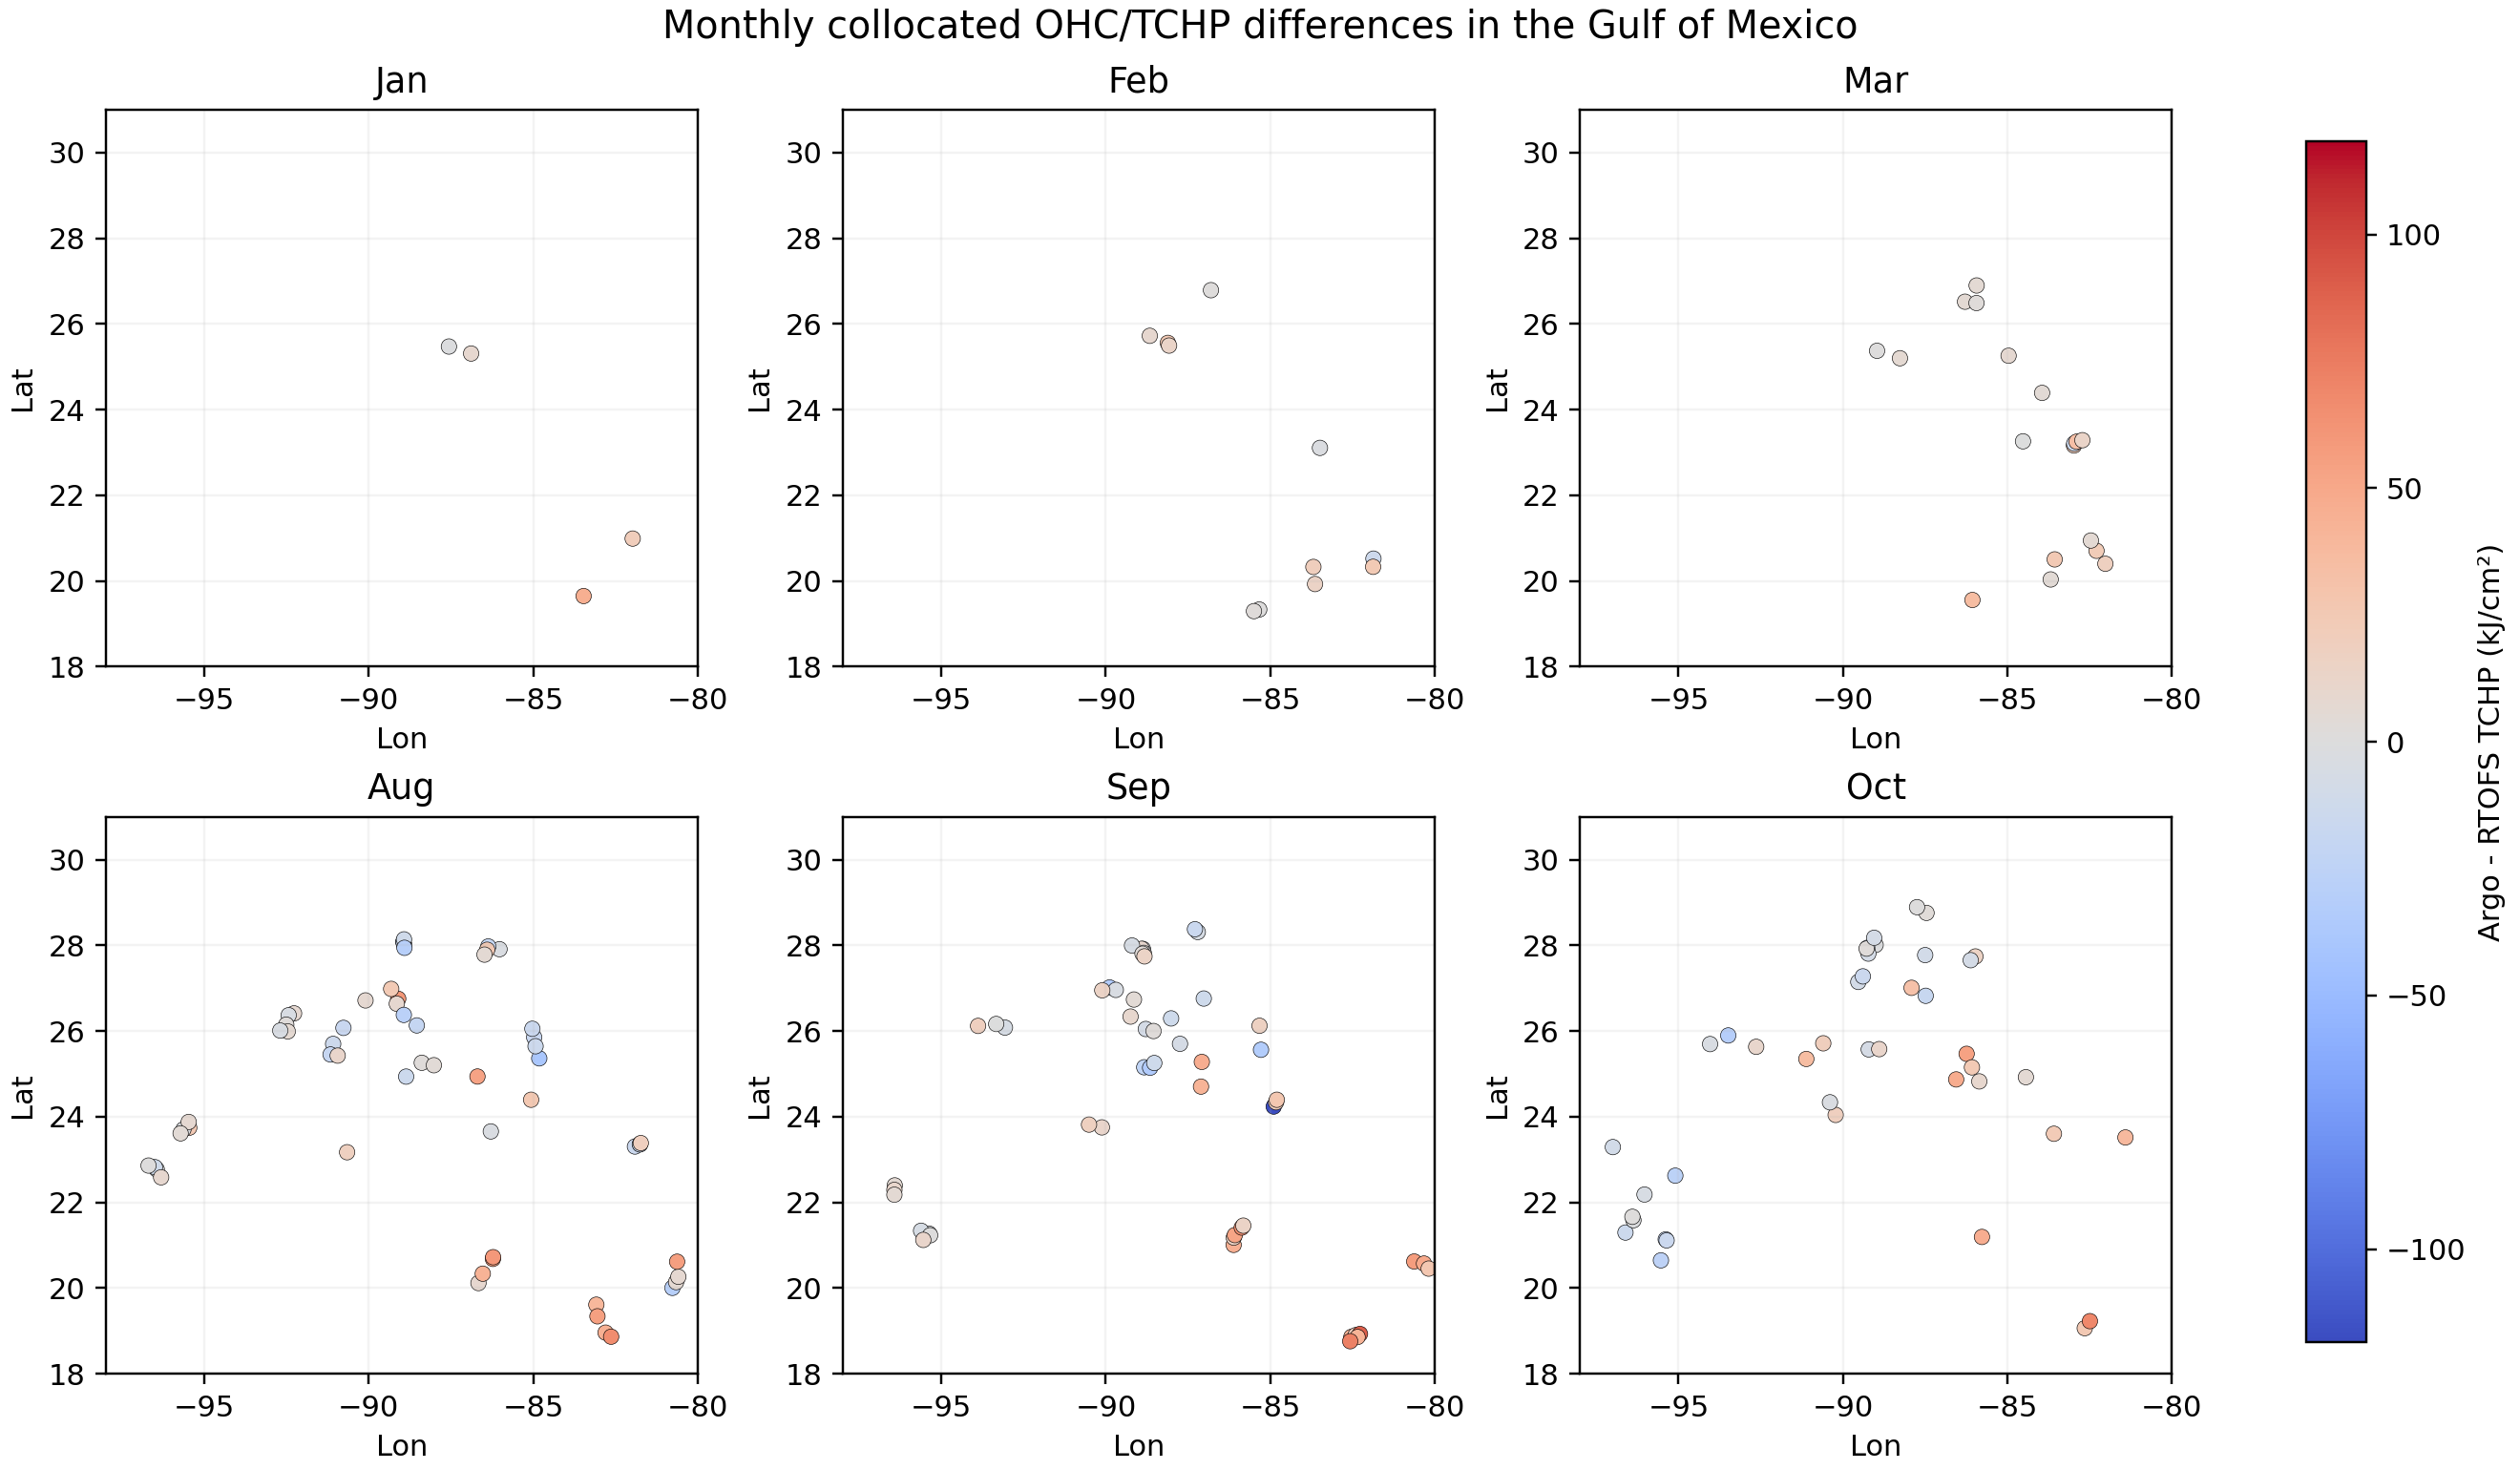
\includegraphics[width=\textwidth]{monthly_difference_maps.png}
\caption{Spatial distribution of collocated monthly differences, computed as Argo minus RTOFS TCHP.}
\end{figure}

\section*{Interpretation}
These monthly means are based on collocated profile dates rather than full-month daily model fields.
That makes the comparison like-for-like at the same locations and times, which is the right framing
for a model-vs-observation OHC benchmark.

\end{document}
